% Multiple Choice Question 5

\begin{center}
    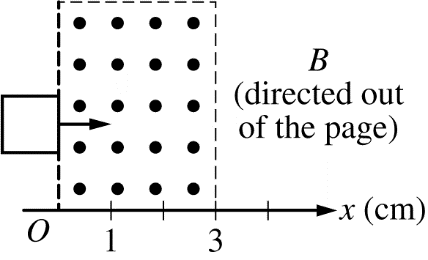
\includegraphics[scale=0.4]{images/img-004-002.png}
\end{center}

\begin{questions}
\setcounter{question}{4}

\question
A square coil with sides of length $1.0\unit{cm}$ is moved through a region of uniform magnetic field at a constant speed, as shown in the figure above. Which of the following graphs best shows the current $I$ in the coil as a function of the position $x$ of the right edge as the coil moves through the magnetic field, where counterclockwise current is positive?

\begin{oneparchoices}
    \choice \adjustbox{valign=t}{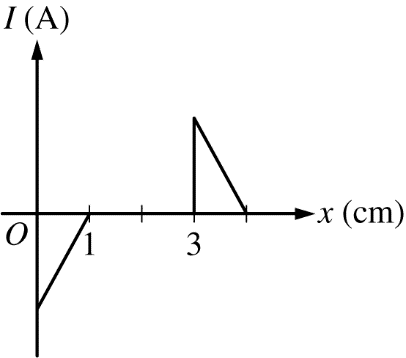
\includegraphics[scale=0.4]{images/img-004-003.png}}
    \choice \adjustbox{valign=t}{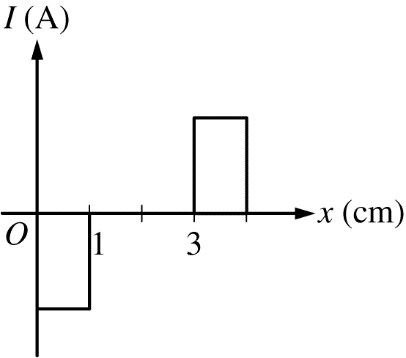
\includegraphics[scale=0.4]{images/img-004-004.png}}
    \choice \adjustbox{valign=t}{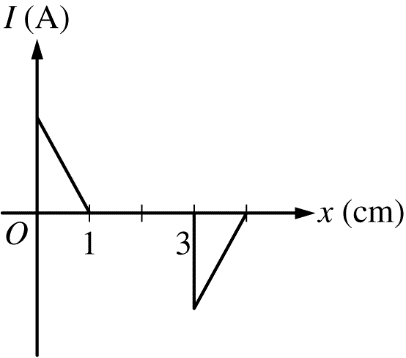
\includegraphics[scale=0.4]{images/img-004-005.png}}
    \choice \adjustbox{valign=t}{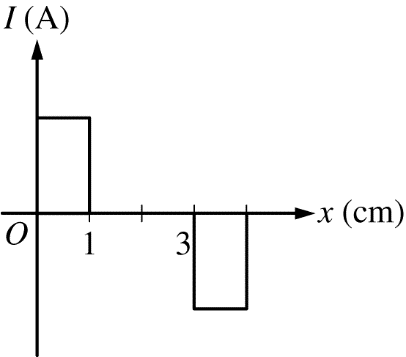
\includegraphics[scale=0.4]{images/img-004-006.png}}
    \choice \adjustbox{valign=t}{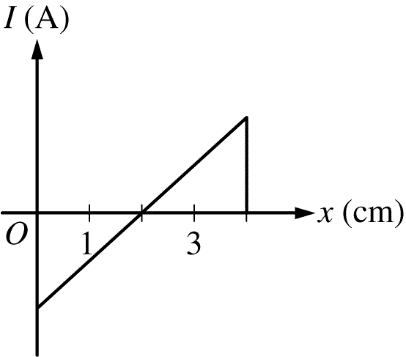
\includegraphics[scale=0.4]{images/img-004-007.png}}
\end{oneparchoices}

\end{questions}
